\documentclass[a4paper,utf8]{article}
\usepackage[heading,fancyhdr]{ctex}
\usepackage{amsmath,amssymb,geometry,lastpage,ulem}
\usepackage{array,tabularx,tabulary,mhchem,xspace}
\usepackage{floatrow,subfig,multirow,bigstrut}
\usepackage{siunitx,booktabs,longtable,graphicx,xfrac,nameref}
\lineskiplimit=1pt
\lineskip=3pt
\geometry{
    top=25.4mm, 
    left=25mm, 
    right=25mm, 
    bottom=25mm,
    headsep=5.9mm,
}
\ctexset{
    section = {format+=\raggedright}
}
\newcommand{\fgref}[1]{图~\ref{#1}\xspace}
\newcommand{\seqref}[1]{式~(\ref{#1})}
\newcommand{\expinfo}[7][无]{
    {\zihao{-3}\bfseries\songti
    实验名称:\uline{\hfill\mbox{#2}\hfill} \\[2.9mm]
    学\quad 号:\uline{\makebox[25mm]{#3}}\hfill
    姓\quad 名:\uline{\makebox[25mm]{#4}}\hfill
    班\quad 级:\uline{\makebox[25mm]{#5}} \\[2.9mm]
    合作者:\uline{\makebox[25mm]{#1}} \hfill
    桌\quad 号:\uline{\makebox[25mm]{#6}}\hfill\makebox[25mm+4em]{}\\[2.9mm]
    实验日期:\uline{\makebox[30mm]{#7}}\hfill\mbox{} \\[58.7mm]
    }
}
\newcommand{\pointingbox}{
    {\zihao{4}\bfseries\songti%
    实验考核\\[3mm]
    \extrarowheight=3mm
    \begin{tabularx}{150mm}{|X|X|X|X|X|}\hline
        \hfil 项目 \hfil  & \hfil 实验预习 \hfil & \hfil 实验过程 \hfil & \hfil 分析与讨论 \hfil & \hfil 总评 \hfil \\[3mm] \hline
        \hfil 评价 \hfil &  &  &  &  \\[3mm] \hline
    \end{tabularx}
    }
}
\newcommand{\derivative}[2]{\frac{\mathrm{d} #1}{\mathrm{d} #2}}
\newcommand{\thinking}[2]{\textbf{#1}\\
答:\begin{minipage}[t]{0.85\textwidth}
    #2
\end{minipage}}
\pagestyle{fancy}
\fancyhf{} \fancyhead[C]{电路基础实验} \fancyfoot[C]{\thepage~/~\pageref{LastPage}}
\newcounter{Rownumber}
\newcommand*{\Rown}{\stepcounter{Rownumber}\theRownumber}
\newcommand*{\resetRown}{\setcounter{Rownumber}{0}}
\newcommand{\qrange}[3]{\qtyrange[range-phrase = \text{$\sim$},range-units =single]{#1}{#2}{#3}}
\floatsetup[table]{capposition=top}
\newcolumntype{C}{>{\hfil}X<{\hfil}}
\renewcommand{\Nameref}[1]{\textbf{\ref{#1}~\nameref{#1}}} %导入导言
\ctikzset{
    resistors/scale=0.7,
    diodes/scale=0.6}
\begin{document}
\begin{center}
    {\mbox{}\\[7em]\zihao{2}\bfseries\songti%
    电路基础实验报告}\\[34mm]
    \expinfo[王慷]{叠加定理}{22301056}{王俊杰}{22 材物}{27}{2024.5.21}
\end{center}
\newpage
\section{实验目的}
\begin{enumerate}
    \item 验证叠加定理。
    \item 正确使用直流稳压电源和万用电表。
\end{enumerate}

\section{实验原理}%简单描述,含必要的公式和附图;
叠加原理不仅适用于线性直流电路,也适用于线性交流电路,为了测量方便,我们用直流电路来验证它。叠加原理可简述如下:\par
在线性电路中,任一支路中的电流(或电压)等于电路中各个独立源分别单独作用时在该支电路中产生的电流(或电压)的代数和,所谓一个电源单独作用是指除了该电源外其他所有电源的作用都去掉,即理想电压源所在处用短路代替,理想电流源所在处用开路代替,但保留它们的内阻,电路结构也不作改变。
\begin{figure}[!ht]
    \subfloat[线性电路]{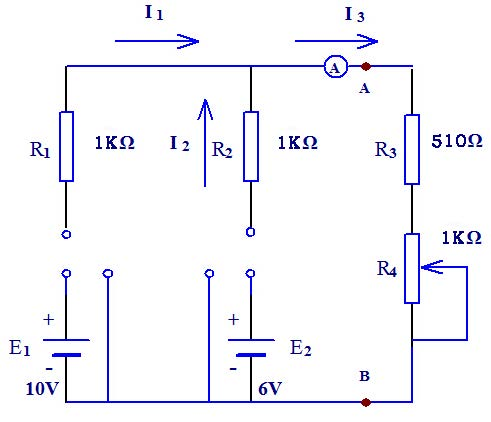
\includegraphics[width=0.45\textwidth]{linear.jpg}\label{fig:linear}}
    \subfloat[非线性电路]{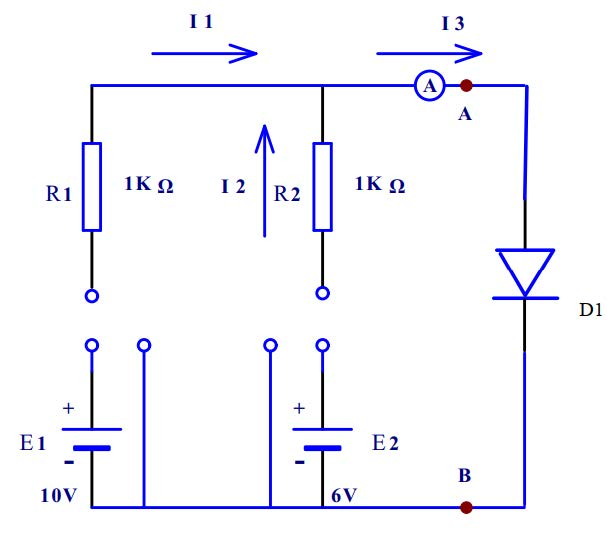
\includegraphics[width=0.45\textwidth]{nonlinear.jpg}\label{fig:nonlinear}}
    \caption{实验所用电路图}
\end{figure}

\section{实验仪表}
    RIGOL DM3058 万用表、RIGOL DP832 直流稳压电源、电路分析实验箱、导线若干。
\section{实验内容}
\begin{enumerate}
    \item 实验箱接通 \SI{220}{\V} 电源,调节直流输出电压,使第一路输出端电压 $E_1 = \SI{10}{\V}$;第二路输出端电压 $E_2 = \SI{6}{\V}$,断开电源开关待用。按图 \ref{fig:linear} 接线, $R_3+R_4$ 调到 \SI{1}{\kilo\ohm},检查线路无误后,再接通电源开关。
    \item 测量 $E_1$、$E_2$ 同时作用和分别单独作用时的支路电流 $I_3$ ,并将数据记入表 \ref{tab:1} 中。
    \item 测量各元件上的电压,将数据记入表 \ref{tab:1} 中。
    \item 将图 \ref{fig:linear} 中 A、B 间的电阻换成二极管,组成如图 \ref{fig:nonlinear} 非线性电路,重复上述步骤,测量数据记入表 \ref{tab:2} 中。
\end{enumerate}
\section{实验结果与分析}
\subsection{实验结果}
\begin{table}[!ht]
    \caption{线性电路测量}\label{tab:1}
    \begin{tabularx}{\textwidth}{c*{4}{C}m{4pt}*{4}{C}}\toprule
        \multirow{3}[2]{2em}{$E_1 E_2$ 作用方式} & \multicolumn{4}{c}{实验测量值} & &\multicolumn{4}{c}{计算值} \\ \cmidrule{2-5} \cmidrule{7-10}
        & $I_3$ & $U_{\text{R}_1}$ & $U_{\text{R}_2}$ & $U_\text{AB}$ & & $I_3$ & $U_{\text{R}_1}$ & $U_{\text{R}_2}$ & $U_\text{AB}$ \\
        & (\unit{\mA}) & (\unit{\V}) & (\unit{\V}) & (\unit{\V}) & & (\unit{\mA}) & (\unit{\V}) & (\unit{\V}) & (\unit{\V}) \\ \midrule
        同时作用 & 5.28 & -4.68 & -0.67 & 5.30 & & 5.33 & -4.67 & -0.67 & 5.33 \\
        $E_1$ 单独作用 & 3.36 & -6.67 & 3.33 & 3.31 & & 3.33 & -6.67 & 3.33 & 3.33 \\
        $E_2$ 单独作用 & 2.02 & 1.99 & -4.00 & 1.99 & & 2 & 2 & -4 & 2 \\ \midrule
        $E_1+E_2$ & 5.38 & -4.68 & -0.67 & 5.30 & & 5.33 & -4.67 & -0.67 & 5.33 \\ \bottomrule
    \end{tabularx}
\end{table}
\begin{table}[!ht]
    \caption{非线性电路测量}\label{tab:2}
    \begin{tabularx}{\textwidth}{c*{4}{C}}\toprule
        \multirow{2}[2]{4em}{$E_1 E_2$ \newline 作用方式} & \multicolumn{4}{c}{实验测量值}\\ \cmidrule{2-5}
        & $I_3$ (\unit{\mA})& $U_{\text{R}_1}$ (\unit{\V}) & $U_{\text{R}_2}$ (\unit{\V}) & $U_\text{AB}$ (\unit{\V}) \\ \midrule
        同时作用 & 14.72 & -9.33 & -5.33 & 0.665 \\
        $E_1$ 单独作用 & 8.76 & -9.33 & 0.640 & 0.642 \\
        $E_2$ 单独作用 & 4.78 & 0.611 & -5.39 & 0.615 \\ \midrule
        $E_1+E_2$ & 13.54 & -8.739 & -4.75 & 1.257 \\ \bottomrule
    \end{tabularx}
\end{table}
\subsection{分析}
在线性电路中,无论是理论计算还是实际测量,$E_1 E_2$ 同时作用的电流和电压都等于 $E_1$ 单独作用和 $E_2$ 单独作用的电流和电压的代数和。而在非线性电路中,$E_1 E_2$ 同时作用的电流和电压并不等于 $E_1$ 单独作用和 $E_2$ 单独作用的电流和电压的代数和,这说明叠加定理只适用于线性电路。
\subsection{误差分析}
    \begin{enumerate}
        \item 万用表在测量电阻时会有内部电阻,这个电阻值会对测量结果产生影响,特别是在测量较小阻值时。
        \item 选择不当的测量范围也可能导致误差,如果选择的范围过大,测量会不准确;如果选择的范围过小,则可能会损坏仪器或导致不准确的读数。此次实验量程为自动确定,不能确定是是否选到了合适的量程。
        \item 温度、湿度等环境因素也会对测量结果产生影响。
        \item 元件长时间摆放导致内部结构发生变化,导致实际值发生变化。
    \end{enumerate}
\subsection{功率能否叠加?}
计算过程如下
\begin{align*}
    p &= (\SI{5.28}{\mA})^2 \times \SI{510}{\ohm} = \SI{14.218}{\mW} \\
    p_1 &= (\SI{3.36}{\mA})^2 \times \SI{510}{\ohm} = \SI{5.7577}{\mW} \\
    p_2 &= (\SI{2.02}{\mA})^2 \times \SI{510}{\ohm} = \SI{2.081}{\mW}
\end{align*}
显然有 $p \neq p_1 + p_2$,故功率不可直接用叠加定理计算,要先用叠加定理计算电流或电压再计算功率。
\section{实验心得}
此次实验使用了 2 个电路来验证叠加定理,在实际操作中,观察到了由于仪器误差和连接线电阻带来的微小偏差,但总体上实验结果符合理论预期。这些实验不仅加深了我对叠加定理的理解,也提升了在实际电路中应用叠加定理的能力。
\clearpage
\section{原始数据}
\begin{center}
    \framebox{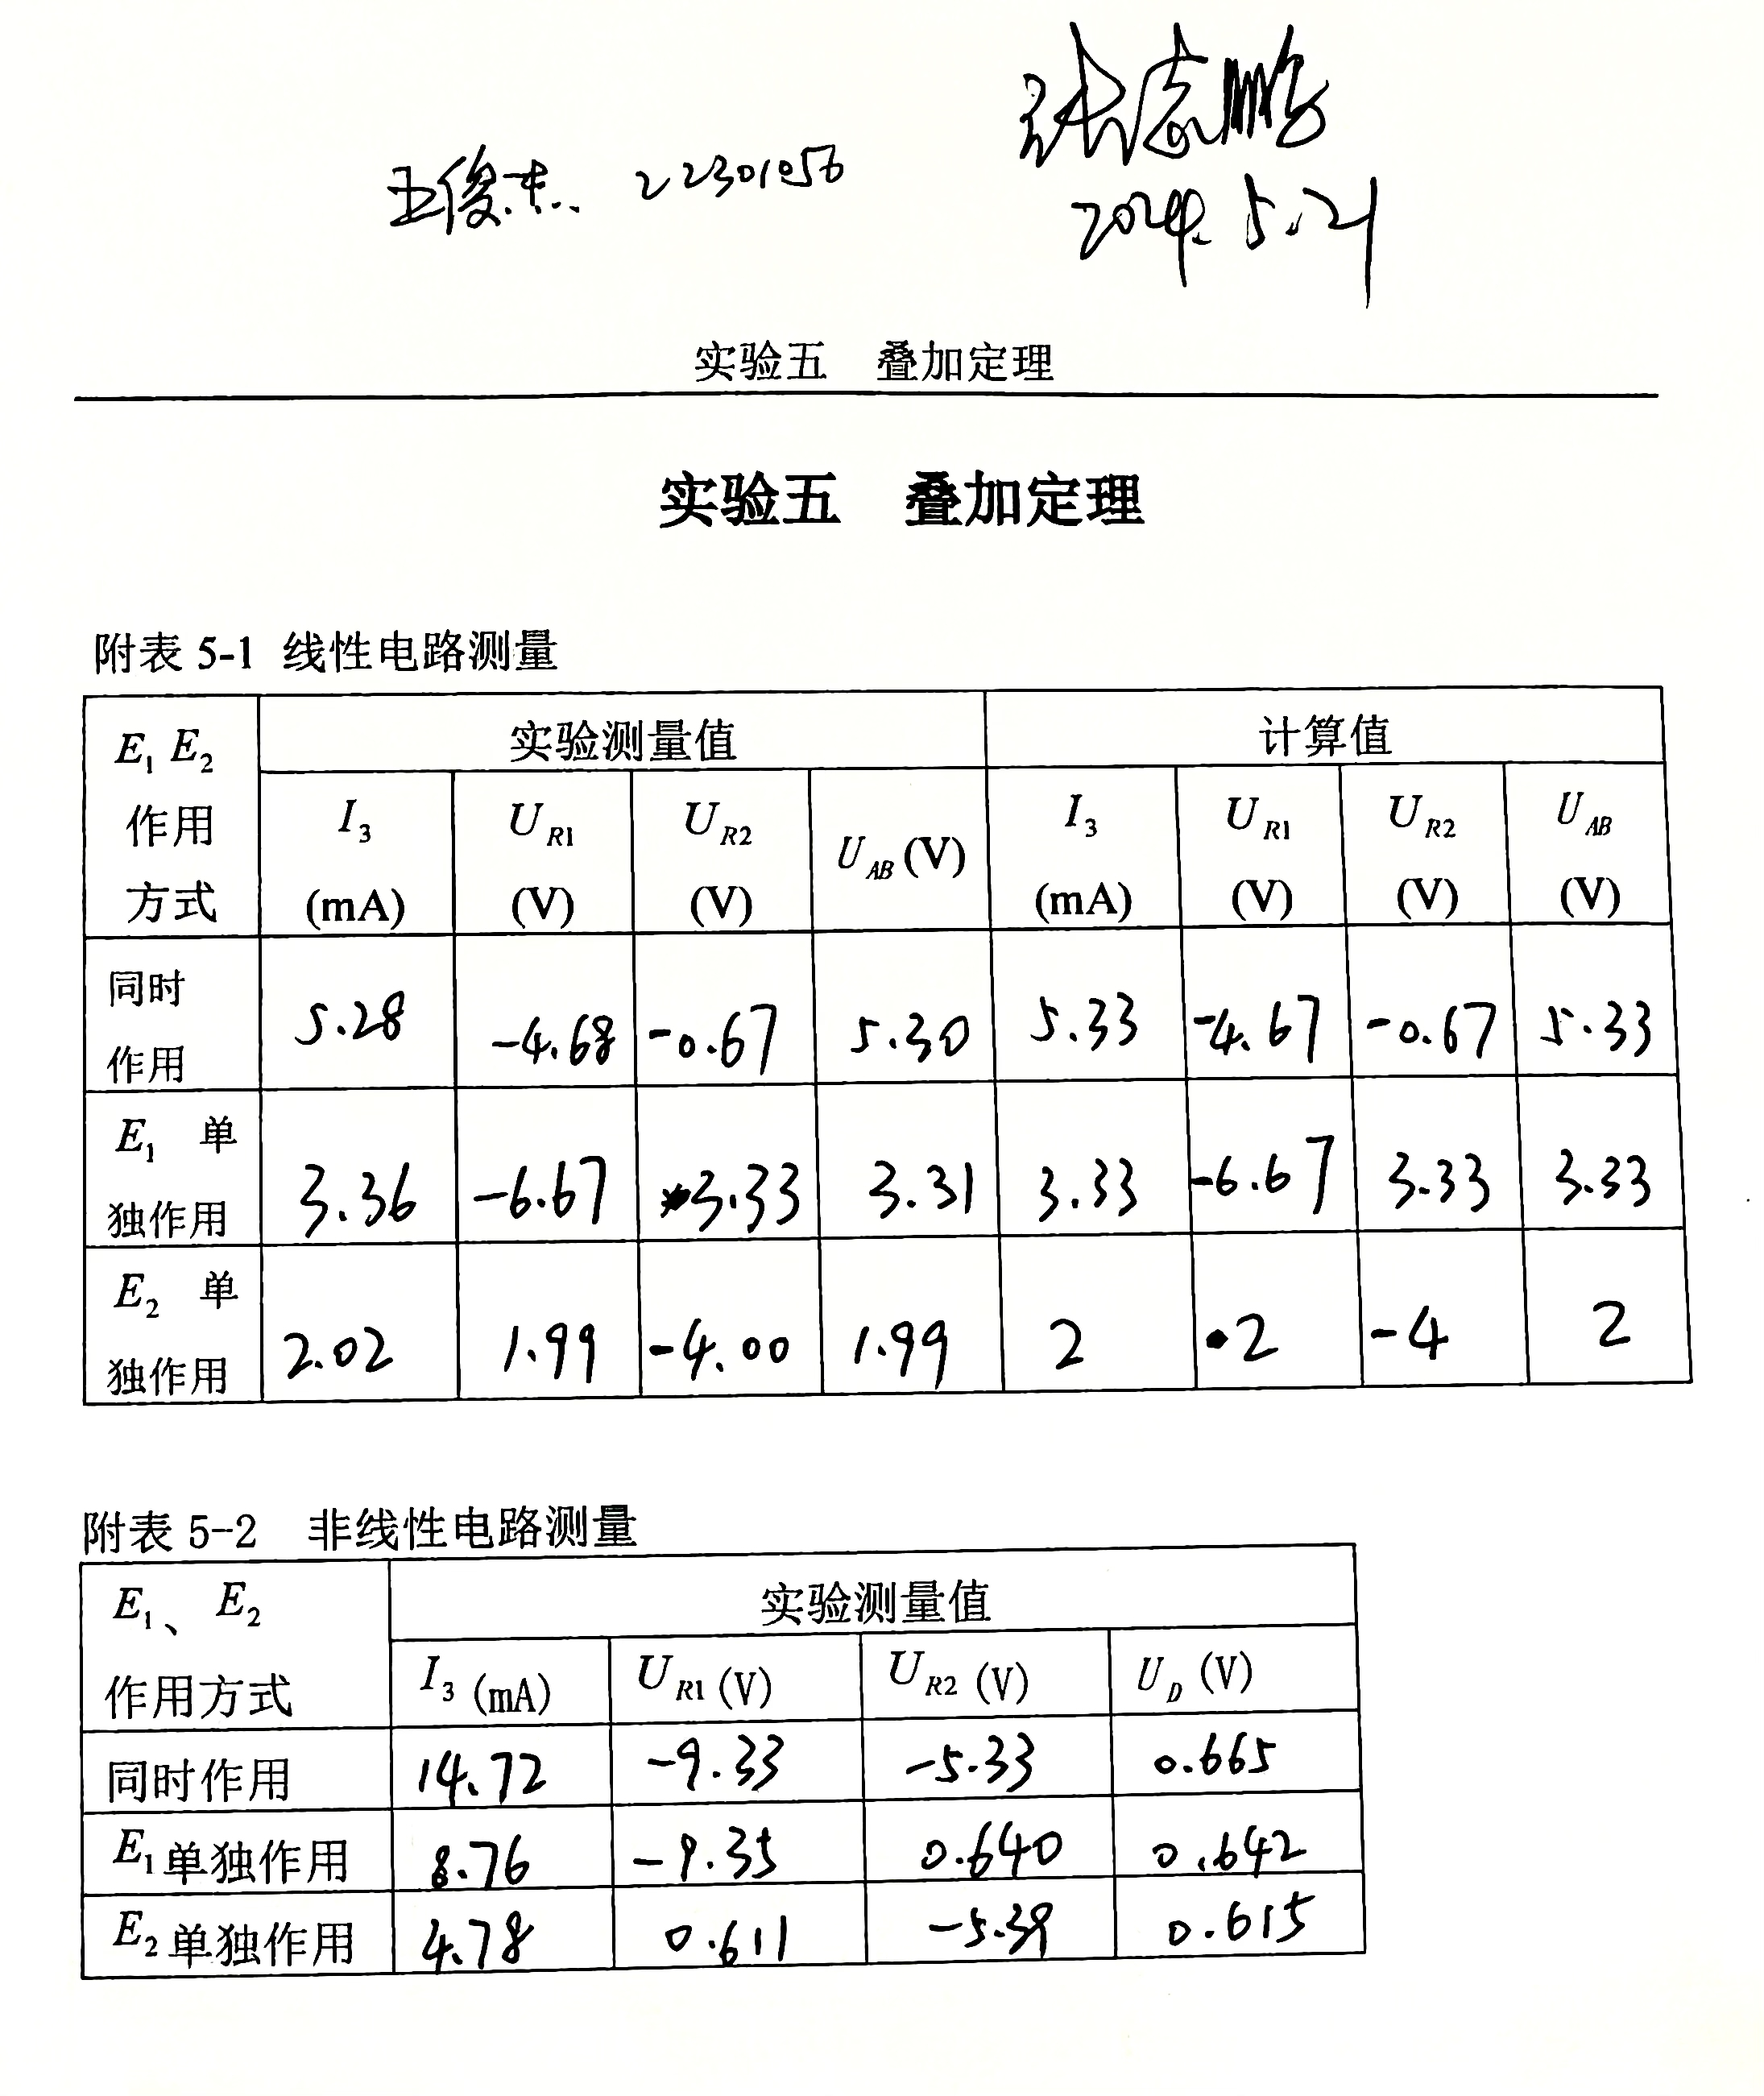
\includegraphics[width=0.95\textwidth]{rawdata.jpg}}
\end{center}

\end{document}